\section{Related Work}
\label{sec:Related Work}

\marginpar{
\begin{itemize}
\item \emph{Which major works consider a similar context?}
\item \emph{Which works are addressing same problem?}
\item \emph{Why are these works insufficient (gaps)?}
\item \emph{Which works use a similar methodology?}
\end{itemize}
}

In this section we present a collection of recent works which are relevant to the problem of autonomous manipulation of articulated objects. Such manipulation tasks are often decomposed into a set of smaller sub-tasks which are solved independently and are unaware of each other. The door opening example already shows which components might be involved. An hypothetical implementation could read as follows. The perception pipeline outputs handle poses from an RGB-D video stream. Once the object pose is established, a manipulation plan is generated. This could be additionally decomposed into a grasping and end effector tracking stages. Usually, a stable handle grasp is seeked and then, a well engineered end effector trajectory is commanded. In this case, the trajectory could be the sequential composition of two arcs, one for unlocking the door mechanism and the other to pull the door open. A low-level end effector controller is then in charge of executing the trajectory by directly commanding the joint torques. As we see in this example, once the door (handle) has been perceived, the perception pipeline is unused. Furthermore a stable grasp assumption could easily fall under slipping and modeling uncertainty. How would then the system know about this failure mode? How would the plan (end effector trajectory) be changed reactively to cope with unforeseen collisions and slipping? While this approach has the advantage of decomposing the complex manipulation in simpler sub-tasks, the resulting framework is purely "open-loop": each module is called only once instead of repeatedly computing the best course of action. This implementation is often referred to as the \emph{sense-plan-act} paradigm ( figure~\ref{fig:sense_plan_act}).     


\begin{figure}[h!]
    \centering
    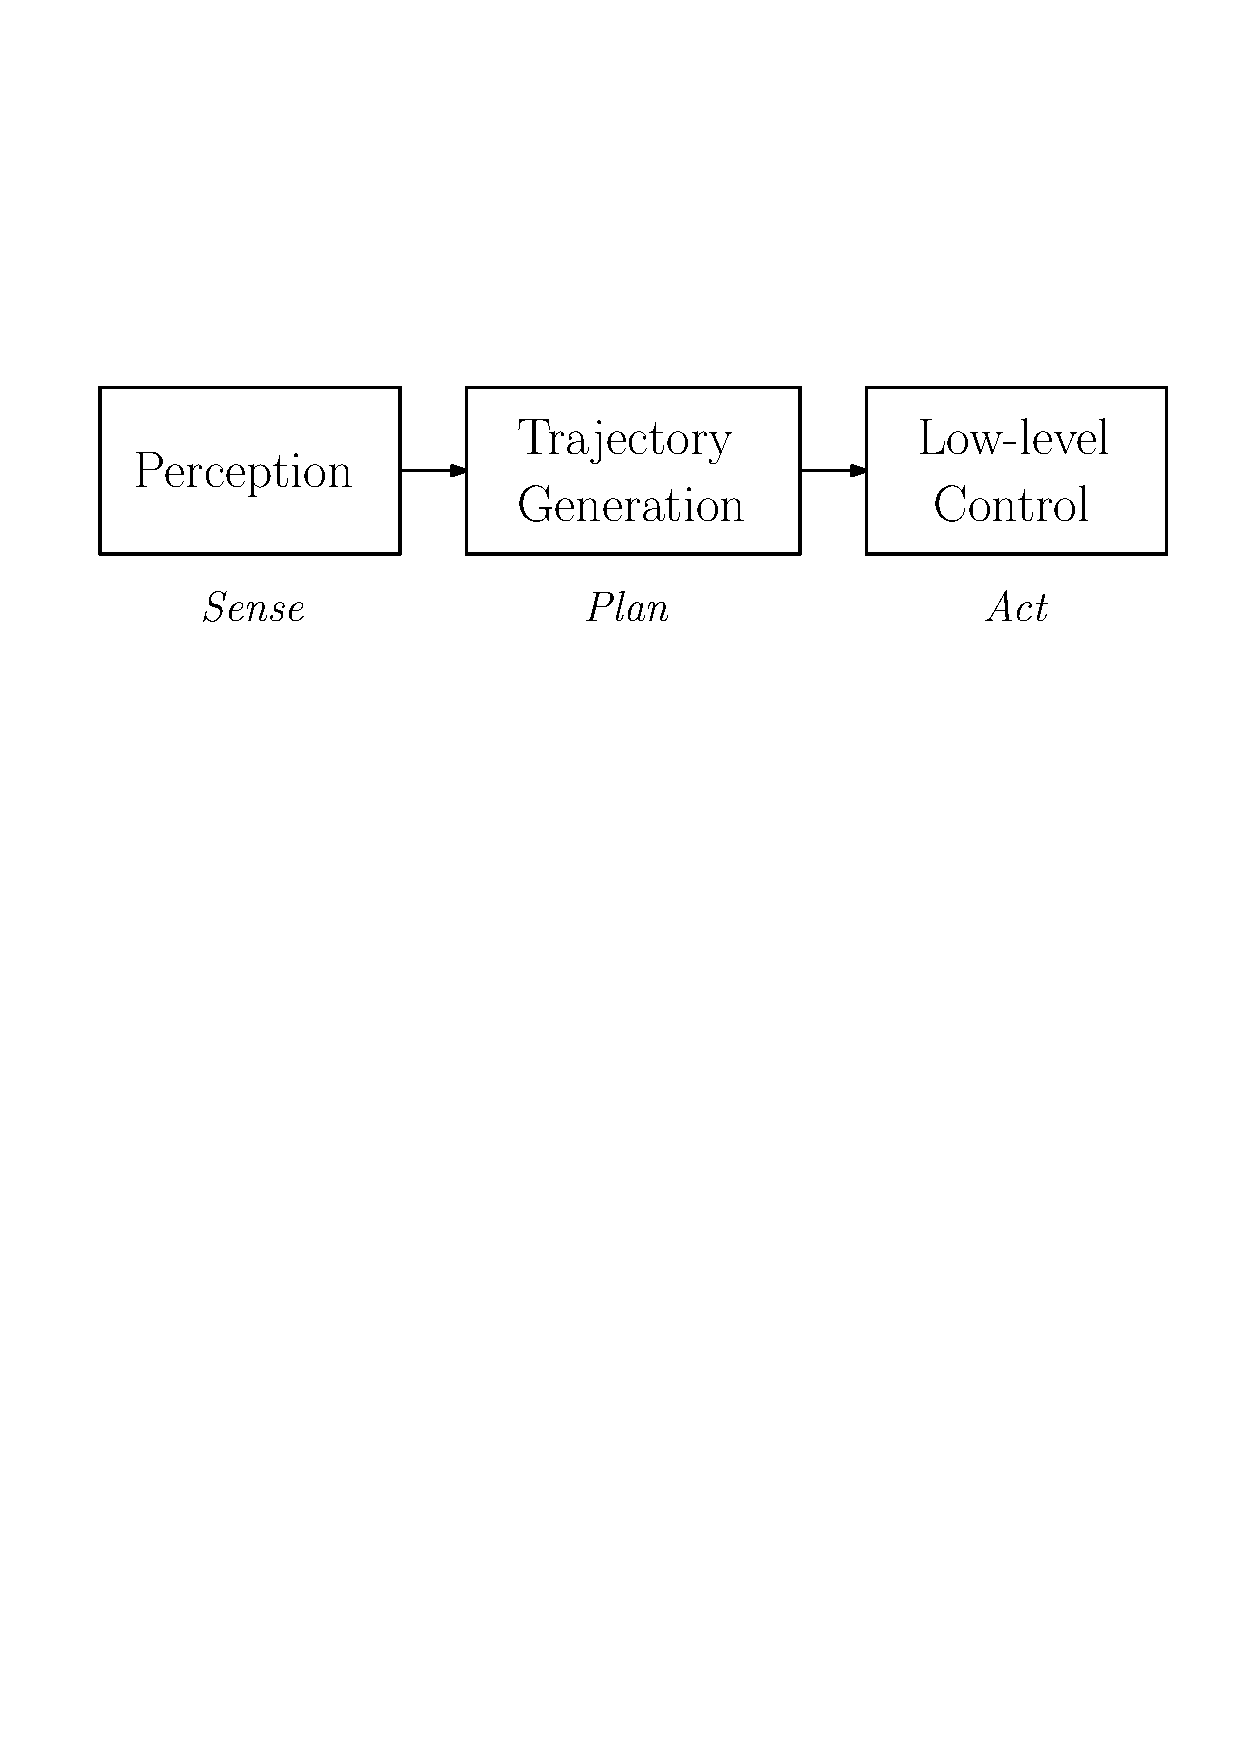
\includegraphics[width=0.6\textwidth]{research_plan/images/sense_plan_act.pdf}
    \caption{The \emph{sense-plan-act} paradigm offers the unique advantage of breaking down the task complexity. On the other hand, information down the stream is never fed back to the sensing and planning modules.}
    \label{fig:sense_plan_act}
\end{figure}

In order to \emph{close the loop} more advanced techniques are deemed. In recent years, the need for advancing platforms and  
algorithms for autonomous manipulation has motivated international robotic challenges such as the Amazon Picking Challenge~\cite{correll2016analysis} (APC) and MBZIRC International Competition ~\cite{baca2020autonomous}. The objective of the APC was to design an autonomous robots to pick up items from a warehouse shelf. In~\cite{cooper2020ari} it is reported that more then 80\% of the 27 participating teams agreed with the statement \emph{perception needs to be better integrated with motion planning}. More then half the participants also agreed with the statement \emph{motion planning needs to be better integrated with reactive planning}. In the extensive and influential review~\cite{bohg2017interactive} the authors claim that a need to bridge teh gap between perception and action in whole-body, multi-contact motion planning and controll is needed. This insightful feedback highlight the need for closing the loop and integrating more perception and planning. In the following we investigate which promising directions have been taken in the fields of perception, modeling, planning and control to address the aforementioned limitation. Furthermore, we envision that the recent technological advance in physical and photo-realistic rendering will play a decisive role in the development of new algorithms. We conclude this section with a brief overview on simulation engines and their potential as core technology for new solutions that span both perception and planning. 

\subsection{Perception}
Perception algorithms are designed to convert raw sensory data (e.g RGBD images and point clouds) into a simpler representation of the scene which can be later used for planning. Ideally, one could directly plan in the space of RGB images~\cite{levine2016end}. Of course this would be extremely complex and is generally addressed by end to end reinforcement learning methods which either requires lots of training data and/or do not generalize well on unforeseen images. Therefore, one has to decide which representation better trades off complexity and representation power. Purely geometric representations of the object as poses~\cite{xiang2017posecnn}, parts~\cite{li2020category} or pixel-wise semantic segmentation~\cite{jang2017end}, provide information about \emph{where} and \emph{what} but not \emph{how}, namely how the object can be interacted with, its function as a part of the whole. Geometrical properties convey just a piece of information required to manipulate an object. We would like a manipulation-oriented perception system which answers the following questions:
\begin{itemize}
\item At which point/part does the interaction happen?
\item What is the function of that point/part?
\item Is the point/part/object movable? If so, how does it move?
\end{itemize}     

Not all questions can be exactly answered by remotely perceiving a static scene. Nevertheless, a perception system could infer a reasonable prior over these properties. For instance, assume that we are looking at a slightly open door which we want to pull completely open. Grasping the handle is only one of the options to successfully executing the task. When we perceive the door, we perceive all the reachable door edges as \emph{actionable points}, namely points we can interact with to successfully reach the desired goal. The perception system is \emph{physically aware}, knows the \emph{physical semantic} of each point on object of interest. This representation has potentially greater within-category invariance. In fact, all doors will share edges and handle shaped links that can be used to pull the door open, independently from their actual visual appearance. The formalization of the above concept goes under the name of \emph{affordances} and was first introduced by the American psychologist James J. Gibson in~\cite{gibson1977theory}. In this seminal work, \emph{affordances} are defined as what the environment \emph{offers} the animal. The hypothesis of affordances can be summarized as follows~\cite{gibson1977theory}:
\begin{displayquote}
\emph{...what we perceive when we look at objects are their affordances, not their qualities; what an object affords us is what we pay attention to while the special combination of qualities into which an object can be analyzed is ordinarily not noticed.} 
\end{displayquote}

This idea has been applied in a number of recent works as an alternative object representation. 
In~\cite{gao2021kpam} the authors develop a perception algorithm which detects semantic 3d-keypoints as the object's representation. Although being a step forward in affordance-based perception, this representation lacks flexibility since it relies on a educated guess (annotation) of interaction hotspots and orientations. Part-based representation allows for a wide generalization across different types of objects as well. In~\cite{myers2015affordance} the proposed approach is able to predict that the bottom of the mug is useful for pounding, or the edge of a turner can used for cutting. A denser representation~\cite{nagarajan2019grounded, mo2021where2act} could be more suited to the task as opposed to lumped positions and orientations. For instance, the autonomous agent might be impaired from reaching the handle while it could easily interact with the door edges. Then it could exploit the knowledge that every reachable point on the edge is interactable in order to find the best interaction candidate. The aforementioned methods provide a dense mapping of affordances but miss the fundamental link with control or collapse the affordance map to poses or single points which are tracked by some off-the-shelf control algorithm. 
We then identify the following unanswered questions:
\begin{itemize}
\item What is the best affordance-based representation for closed-loop manipulation control? 
\item How can we directly plan in the space of affordances?
\end{itemize} 
 
\subsection{Modeling}
Once an interaction is engaged, the robot needs to determine the outcome of its actions and how they change the environment. In the context of articulated objects this means that the it needs to estimate the object articulation mechanism, implemented as a kinematic constraint. Kinematic constraints are generally represented using different articulation models, e.g. revolute or prismatic. Many recent works have focused on extracting the articulation model category and its parameters from a static scene~\cite{abbatematteo2019learning, li2020category}. 
Passively perceiving the environment can provide good prior knowledge for modeling the scene, however the accuracy of such model is limited by the sensor capabilities and can be deteriorated by sensor noise, occlusions, limited field of view and intrinsic ambiguities. While precise modeling is required to successfully act in the environment, acting can provide even more precise information about the environment itself. The latter approach is referred to as \emph{active perception}. Following the definition in~\cite{bajcsy2018revisiting}:
\begin{displayquote}
\emph{An agent is an active perceiver if it knows why it wishes to sense, and then chooses what to perceive, and determines how, when and where to achieve that perception.}
\end{displayquote}  
As an example, an information gain criteria is often used to steer perception toward more informative area (citations). When the policy considers interactions and explicitly uses them to gain more information, then we talk about \emph{interactive perception}~\cite{bohg2017interactive, katz2014interactive}. For example, the robot may not know whether two objects are rigidly connected or simply in contact; interactive perception allows to test each hypothesis by applying forces on the scene and observing the resulting object configuration~\citep{kroemer2019review}. 

Interactive perception often relies on priors in order to simplify the estimation problem. In fact, computing a posterior without any prior on the object category (deformable vs rigid) and articulation model (revolute vs prismatic) is instractable. Instead most systems rely on some previous knowledge. Often, the perception system is able to provide a good prior about the articulation model~\cite{katz2011interactive} and we know a priori that the object of interest is articulated and not deformable. Most approaches impose some structure on the type of the interaction. They often rely on a rigid grasp model \cite{karayiannidis2013model} and a set of action primitives such as pull, push, grasp which are assumed to be executed without failure~\cite{hausman2015active}. An implicit assumption that is made in this works consists in the access to nicely shaped handles that generally stand out from the object surface. It is not clear how these approaches would work for an embedded handle as the one shown in figure \ref{fig:dishwasher_handle}

\begin{figure}[h!]
    \centering
    
\includegraphics[width=0.6\textwidth]{research_plan/images/dishwasher_handle.png}
    \caption{Traditional household furniture has handles which do not always allow to easily close the grasp on both sides. In this cases, it is harder to ensure a fixed grasp and planning interaction results consequently more complex.}
    \label{fig:dishwasher_handle}
\end{figure}


During interactive perception, multiple sensor modalities can be combined: the already mentioned RGBD and time of flight sensors and also haptic devices such as force-torque cells. How to combine these modalities optimally is still an open question. In fact, more sensors introduce also more noise and complexity. Furthermore, we can only partially observe the state of the world. A reasonable question is then, how can we cope with uncertainty? If we maintain a full distribution over the quantity of interest, then computing an action that takes uncertainty into account is usually intractable~\cite{lavalle2006planning}.In general, we are not interested to identify the model parameters per se but rather to achieve the manipulation goal. A better estimate of the model and its parameters is then functional as long as the objective is executed better and faster.   

\subsection{Planning}
Manipulating an object involves a wide range of motions that is hard to achieve with fixed base manipulators. For this reason, they are often combined with a mobile base for greater mobility and unconstrained workspace. As an example, the rotation range of the door could be too big to be handled by a fixed base arm while fulfilling joint limits constraints. However, to fully exploit these capabilities, systems require planning algorithms that can generate fast, accurate and coordinated reactive whole-body motions that account for multiple potential contacts with the environment. While traditional ``plan-and-act'' frameworks break down such tasks into subproblems that are easier to solve (e.g. reach, grasp, pull)~\cite{Murali2020}, they do not offer fast and control-aware replanning, which is crucial for mobile manipulation  in dynamic and uncertain environments. 
With the recent advancements in artificial intelligence, reinforcement learning is a promising method to solve a range of robotic control tasks, including manipulation~\cite{finn2016deep}, as they learn an end-to-end representation of the optimal policy. However, real-world applications of reinforcement learning typically require training times that are not practical for physical hardware and suffer from the well-known \emph{sim-to-real} gap~\cite{chebotar2019closing}. 
On the other side of the spectrum, Model Predictive Control (MPC) has gained broad interest in the robotics community thanks to its capability of dealing with input constraints and task objectives by solving a multivariate optimization problem. 
MPC has been successfully applied to aerial robots~\cite{brunner2020trajectory}, autonomous racing~\cite{liniger2015optimization}, legged locomotion~\cite{grandia2019frequency} and whole-body control~\cite{minniti2019whole}. Nevertheless, MPC requires a model that is locally differentiable with respect to the input and the state~\cite{buchli2017optimal}. On the other hand, manipulation tasks involve changes in the contact state causing sharp discontinuities in both the cost and system dynamics, thus directly violating the differentiability requirements. 

Recently, sampling-based methods have emerged and advanced in theory and applications~\cite{lee_aggressive_2020,abraham_model-based_2020,rajamaki_augmenting_2017}. 
In contrast to traditional MPC, sampling methods stem from a probabilistic interpretation of the control problem. 
Rather than solving a big optimization, they rely on sampling system trajectories. The only requirement is that it is possible to forward simulate the system evolution. This has been exploited to control camera motions for target tracking in drone racing~\cite{lee_aggressive_2020}, robot arm motions for manipulation tasks~\cite{abraham_model-based_2020} and for generating aggressive driving maneuvers such as drifting~\cite{williams_information_2017}. 

Yet despite their appealing features, sampling-based methods can be costly to execute and solution quality is highly dependent on sampling quality. Previous works argue that thousands of trajectories need to be sampled in real time for the effectiveness of the proposed sampling-based algorithm and therefore GPU-based simulation is needed for fast parallel computation~\cite{williams_model_2017}. Unfortunately, GPUs are not common on mobile robots (e.g., because of limited power and payload) and the overall computation times are often not adequate for feedback control. 
Furthermore, demonstrated solutions for tasks involving different physical interactions (e.g. a robot arm opening a drawer~\cite{abraham_model-based_2020}) have been shown on a real system only by breaking down the multi-contact task into stages and enforcing constraints when switching between them. 
This can limit the control envelope of the system and sacrifices solution optimality. For example, it is common practice to fix the gripper orientation between successive reach and pull stages and perform manipulation under a rigid grasp. In the presence of uncertainty and tracking errors, this often leads to high contact forces that might damage the robot as well as the manipulated object.
Ultimately, because of the lack of practical implemented solutions, sampling-based control methods are yet to be applied on real mobile manipulators for whole-body control of complex multi-contact tasks.   


\subsection{The Rise of Simulators}
We expect that perception, planning and model estimation algorithms could greatly profit from the readiness level of physics and sensor rendering capabilities reached nowadays.  
In recent years, simulators have covered a fundamental role in robotics research. Simulators allow to validate control strategies without access to real-world hardware. Many instantiations of a simulation can run in parallel and are often faster than real-time. Data-hungry deep learning approaches heavily employ simulators as a cheap source of data for training while obviating the potential damage to the robot~\cite{liang_gpu-accelerated_2018}. However, there are discrepancies between simulations and the real world. Certain physical phenomena such as gear backlash, sensor noise and latencies are approximated or removed. This prevents control systems created in simulation from performing to the same standard as in reality \cite{collins_benchmarking_2020}. This disparity is known as the \emph{reality gap}~\cite{hofer2021sim2real}. In order to reduce the impact of the reality gap, physical parameters are then sampled and modified between multiple simulation runs. As a result, the control policy is more robust to real world variations when transferring it to the real-robot~\cite{andrychowicz2020learning}. This technique, called \emph{domain randomization} has pushed simulators to expose in their API methods to dynamically change physical and geometrical properties such as friction, damping, mass, joint axis position and orientation, collision and visual meshes. (express that this capability can be deployed in a real time setting) 

(more citations, second part is especially unclear)
Nevertheless, contemporary simulators have achieved a level of accuracy and speed that make them not only appealing for offline data collection but also for real-time deployment as a model of the system dynamics. This is particularly important for manipulation as physics engines can reliably predict the outcome of complex interactions in faster-than-real-time. Nevertheless, most approaches still use simulation only for validation or data generation. (move this to the rl part)From the learning perspective this means that the learning agent can reach at most the same accuracy as the simulator. Furthermore, the bad performance of these algorithms on the real platform is a result of the intertwined controller behavior, which can be by its own suboptimal, and modeling mismatch.   
